% !TeX spellcheck = cs_CZ
\wikitextrule
\begin{example}\label{MAI:exam019} 
  Funkce je dána vzorcem 
  \begin{equation*}
    f(x):y=\abs{x}.
  \end{equation*} 
  Přirozeným definičním oborem této funkce je množina $\realset$. Táž funkce může být dána i 
  vzorcem
  \begin{equation*}
    f(x):y=\sqrt{x^2},
  \end{equation*}    
  nebo dvěma rovnicemi
  \begin{equation*}
    f(x):y=
       \begin{cases}
           x & \text{je-li} x \geq 0. \\
          -x & \text{je-li} x < 0,
       \end{cases}                 
  \end{equation*}  
  což je zřejmé, uvědomíme-li si jak je definována absolutní hodnota. Graf funkce je na obr. 
  \ref{mai:fig007}.
  
  {\centering
   \captionsetup{type=figure}
%  % !TeX spellcheck = cs_CZ
% mai_fig007.tex

\documentclass[11pt]{standalone}
\usepackage{xltxtra}
\usepackage[usenames,x11names]{xcolor}
\usepackage{tikz}
\usepackage{pgfplots}
  \pgfplotsset{compat=newest}
\usepackage{amsmath}

\begin{document}
  \begin{tikzpicture}[thick,scale=0.7, every node/.style={transform shape}]
    \begin{axis}[
      xmin = -3, xmax = 3, ymin = 0, ymax = 3,  % osy
      domain = -3:3,
      restrict y to domain=0:3,
      grid = major,   % both
      grid style={line width=.1pt, draw=gray!20},
      major grid style={dashed, line width=.2pt, draw=gray!40},
      minor tick num=5,
      clip = true,
      clip mode=individual,
      axis x line = middle,
      axis y line = middle,
      xlabel={\(x\)},
    %  xlabel style={at=(current axis.right of origin), anchor=west},
      ylabel={\(y\)},
    %  ylabel style={at=(current axis.above origin), anchor=south},
      enlarge y limits={rel=0.13},
      enlarge x limits={rel=0.07},
    ]
    
     \addplot[color=Gold3, samples=200, smooth, ultra thick, unbounded coords=jump, no markers] 
        gnuplot{abs(x)};  
    \end{axis}
  \end{tikzpicture} 
\end{document}
   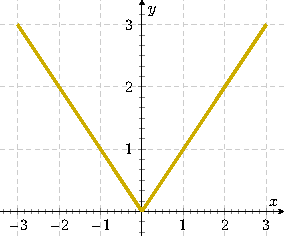
\includegraphics[width=0.5\linewidth]{mai_fig007.pdf}
   \captionof{figure}{Graf funkce $y=\abs{x}$}
   \label{mai:fig007}
  \par}
\end{example}